\documentclass[twocolumn,11pt]{article}
%\documentclass[10pt]{article}
\usepackage[top=1in, bottom=1in, left=1in, right=1in]{geometry}
\geometry{letterpaper}
%\geometry{landscape}
\usepackage{multicol}
%\usepackage[parfill]{parskip}
\usepackage[parfill]{parskip}

\usepackage{fancyhdr}
\pagestyle{fancy}
\usepackage{url}

\usepackage{graphicx}
\usepackage[leqno]{amsmath}
\usepackage{amssymb}
\usepackage{epstopdf}
\DeclareGraphicsRule{.tif}{png}{.png}{`convert #1 `dirname #1`/`basename #1 .tif`.png}

\renewcommand*\thesubsection{\arabic{section}\alph{subsection}}

%\usepackage{qtree}
%\usepackage{subfigure}

% I prefer symbols to numbers for footnotes.
\renewcommand{\thefootnote}{\fnsymbol{footnote}}

% funky Dartmouth imod command, uses less horizontal space: a\equiv b \imod c
\makeatletter
\def\imod#1{\allowbreak\mkern10mu({\operator@font mod}\,\,#1)}
\makeatother

\usepackage{enumitem}
\usepackage{caption}
\usepackage{subcaption}

\usepackage{float}
%\usepackage[nomarkers,tablesonly]{endfloat}

\usepackage{listings}
\usepackage[usenames,dvipsnames]{color}
\usepackage{courier}
\usepackage[table]{xcolor}
\definecolor{notepad}{cmyk}{0.0,0.0,0.25,0.0}
\definecolor{screen}{cmyk}{0.0,0.0,0.00,0.10}
\definecolor{greenScreen}{rgb}{0.0,1.0,0.0}
\lstset{
	basicstyle=\fontfamily{pcr}\selectfont\footnotesize,
%	numbers=left,
%	numberstyle=\footnotesize,firstnumber=1,
	stepnumber=1,
%	numbersep=10pt,
	backgroundcolor=\color{notepad},
	showspaces=false,
	showstringspaces=false,
	showtabs=false,frame=single,
	tabsize=4,
	captionpos=t,
	breaklines=true,
	breakatwhitespace=false,
	escapeinside={\%*}{*)} % if you want to add a comment within your code
}

%---------------------------->8   header crap   >8------------------------------

\lfoot{Collier}
\rfoot{Stat E-104}
\lhead{}
\rhead{Page \thepage\ }
\cfoot{Top Kaggler}

\title{Top Kaggler\\STAT E-104 Project}
\author{Jeff Collier\footnote{but on Kaggle they call me Maurice}}
\date{4 MAE 2015}

\begin{document}
\maketitle

%-------------------------->8   And we're off   >8------------------------------

\section*{The Challenge}
Given some data on home sales, we're to demonstrate our ability at modeling using linear regression.
Building on that, use the model to estimate the prices of houses represented by a smaller set of data
as part of a challenge.

The only real trick to cooking is to pick good ingredients and make sure you don't screw them up.
One mantra from the TV series Top Chef is if it didn't work, don't serve it.
I have a feeling those may be conflicting goals modeling these data.
Still, they are the guidelines that will inform my actions.
That said, let's take a look at what we have in the pantry.

%----------------------------->8   Section   >8---------------------------------

\section*{The Data}
The data is described in Table~\ref{tab:data}.
I renamed some of the original variables because \LaTeX{} sucks at random underscores.
One of the first steps to a regression analysis is to look at each variable.
I'll break the data up into groups and get a taste of each of them individually.

%--

\subsection*{salesprice, pl}
Let's start with a taste of what we are trying to predict, $salesprice$.
Some strong hints and exploratory regressions
indicated that transforming $salesprice$ might be a good idea.
Stata's reports via detailed summary that the skewness of $saleprice$ is $>0.97$;
this is greater than our $0.8$ rule of thumb for requiring transform.
Regression estimates are really the mean of a normal distribution.
If the actual underlying data is skewed, our estimate are more likely to be more off.
It was nigh on impossible to get exploratory regressions of $salesprice$ to pass Stata's $sktest$.

We see from Figure~\ref{fig:salesprice-box} that
$salesprice$ is skewed towards larger values and has a few outliers.
We will leave outliers in the mix for now:
removing them would restrict the range of values we could predict for.

Given that it is likely we'll need to eventually transform $salesprice$
we will use $pl = ln(salesprice)$ as our dependent variable going forward.
We see from Figure~\ref{fig:pl-qnorm}\footnote{This plot gives
us a line that, if the distribution were normal, the scattered points would fall on or near.}
that a natural log transform gives us a roughly normal fit.

This will force us to adjust our interpretations of the coefficients\footnote{I learned what
I know of this from  \url{"http://www.biostathandbook.com/transformation.html"} but all misunderstandings are my own.}.
Using the log means coefficients represent the percentage change in our dependent variable based on change in the predictor.
But this is better than restricting the range of values our model can reasonably predict for.
\begin{figure}[H]
\centering
  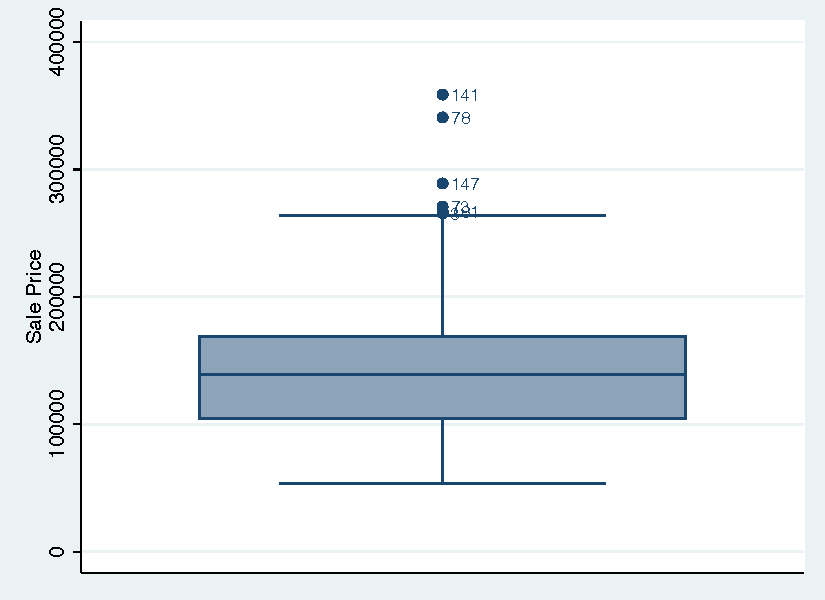
\includegraphics[width=.9\linewidth]{figures/salesprice-box.pdf}
  \caption{salesprice}
  \label{fig:salesprice-box}
\end{figure}
\begin{figure}[H]
  \centering
  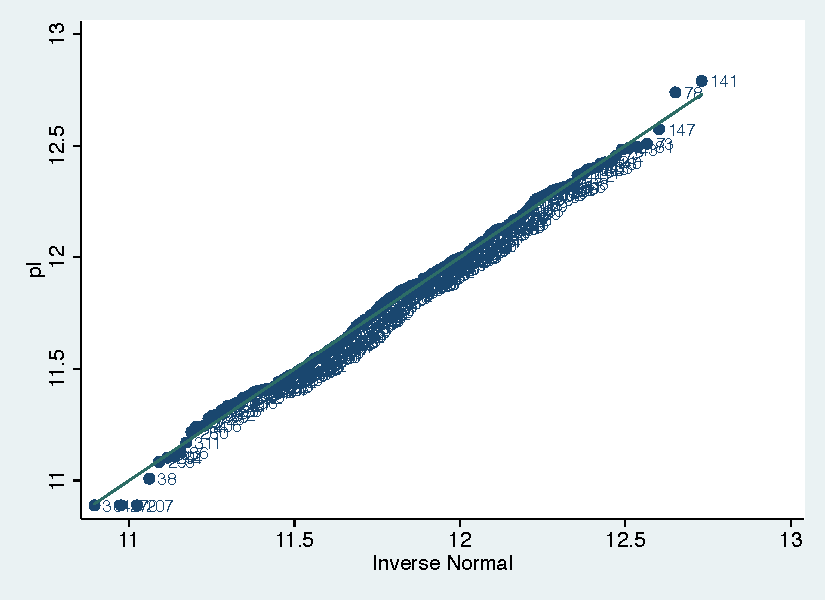
\includegraphics[width=.9\linewidth]{figures/pl-qnorm.pdf}
  \caption{Transformed Sales Price}
  \label{fig:pl-qnorm}
\end{figure}

%--

\subsection*{Month Sold}
Month sold would seem to be a better predictor of volume of sales, not price.
Examining sales price by month in Figure~\ref{fig:uniMonth}
shows a more uniform distribution of sales price.
Both the middle 50\% of the price of homes sold and the remaining data
all overlap to some degree, many to a large degree.
I plan on ignoring this variable.
\begin{figure}[H]
\centering
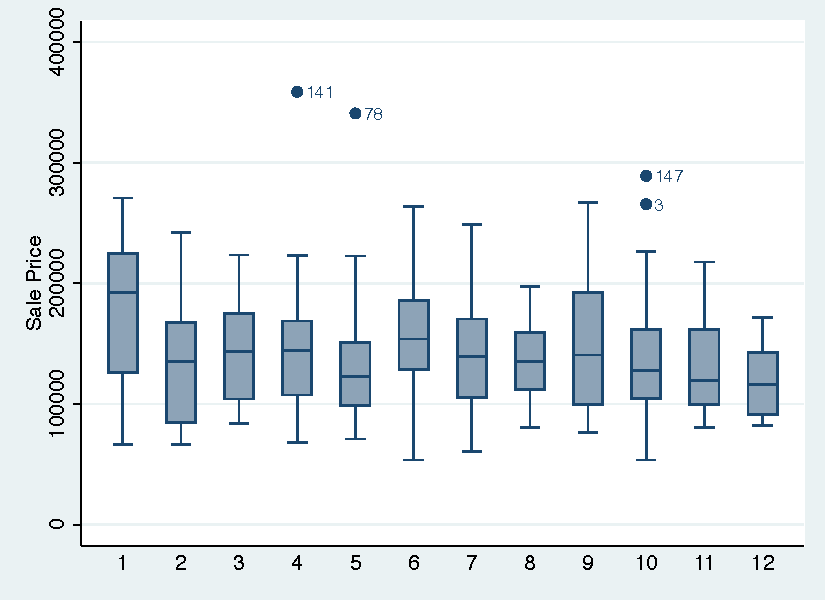
\includegraphics[width=.9\linewidth]{figures/uniMonth.pdf}
\caption{Sales price by month sold}
\label{fig:uniMonth}
\end{figure}
\begin{figure}[H]
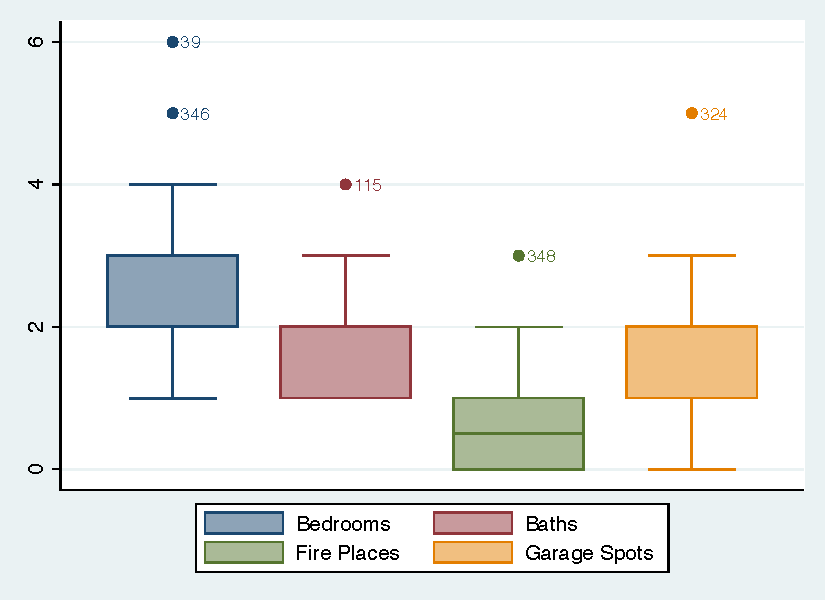
\includegraphics[width=.9\linewidth]{figures/uniCats.pdf}
\caption{Bedrooms, baths, fire places, garage spots}
\label{fig:uniCats}
\end{figure}
\begin{figure}[H]
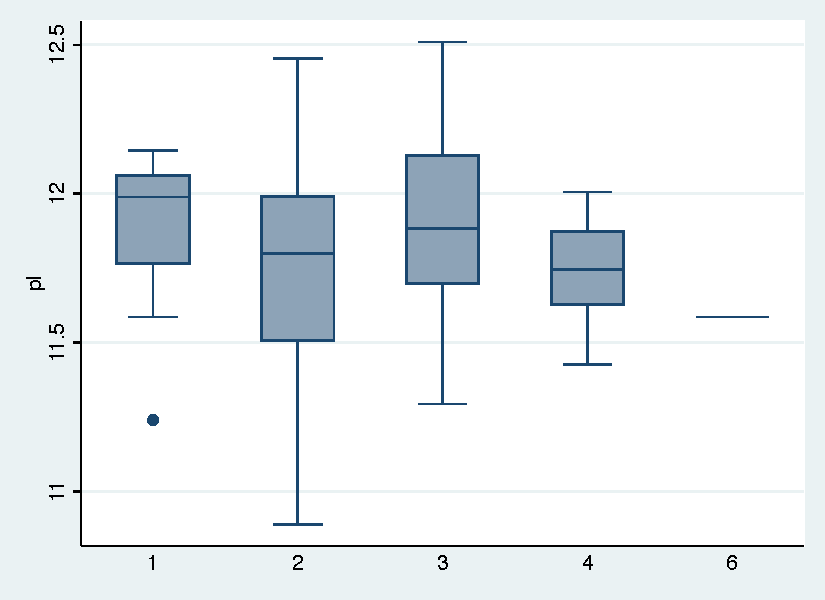
\includegraphics[width=.9\linewidth]{figures/br-box-wow.pdf}
\caption{Variance of pl over bedrooms}
\label{fig:br-wow}
\end{figure}

%--

\subsection*{The Counts}
Baths, bedrooms, fire places and garage spots:
these counts would all seem likely predictors of sales price, worth the trouble of mining.
I expect that the sale price would increase as these values increase.
But Figure~\ref{fig:uniCats} shows that there isn't much variance in these data.
Also, the distribution fire places is skewed, so I added an indicator variable, fpp, if it has one or more.
Bed rooms is also a curiosity: observe the variance of pl over each value in Figure~\ref{fig:br-wow}.
This explains why this variable had a negative coefficient in exploratory regressions.

%--

\subsection*{Age}
Age is a continuous variable that negatively affects the price of the house, as seen in Figure \ref{fig:ageScatter}.
Transforming by ln only seems to have traded one curve for another (Figure~\ref{fig:agetScatter}),
but exploratory regressions using the two different variables show that while $age$
doesn't pass Stata's ovtest and hettest for linearity and heteroscedasticity,
$aget$ is suitable for regression on its own.
\begin{figure}[H]
\centering
  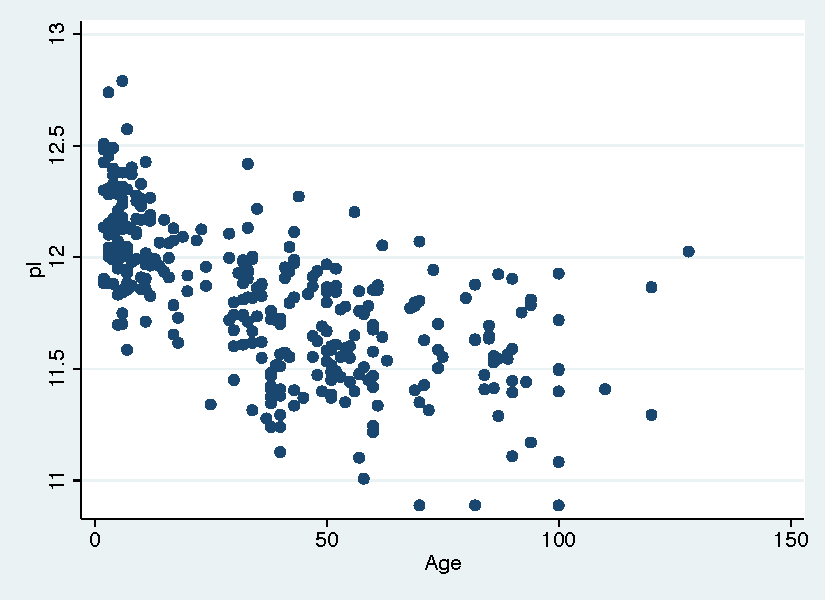
\includegraphics[width=.9\linewidth]{figures/age-scatter.pdf}
  \caption{Curvy scatter of Age}
  \label{fig:ageScatter}
\end{figure}
\begin{figure}[H]
\centering
  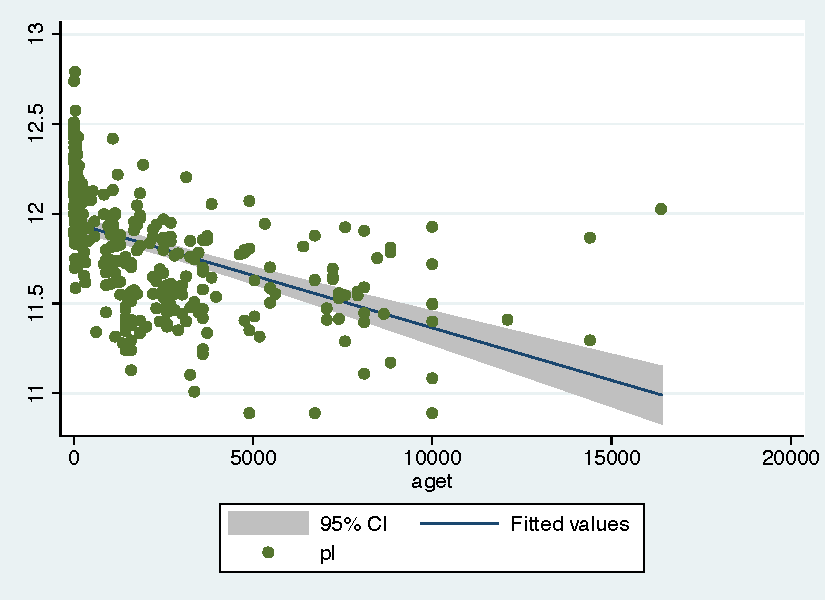
\includegraphics[width=.9\linewidth]{figures/aget-scatter.pdf}
  \caption{Curvy scatter of transformed Age}
  \label{fig:agetScatter}
\end{figure}

%--

\subsection*{Central Air Conditioning}
While most homes have this, there is clearly a differential in the Figure~\ref{fig:cac-box}.
This was confirmed by a two sample t-test.
Given $H_0: \mu_{cac=1} = \mu_{cac=0}; H_a: \mu_{cac=1} > \mu_{cac=0}$ resulted
in $p < 0.0001 $ which means we reject the null hypothesis; homes with central air sell for more.
This could be a useful indicator variable but only five of $319$ homes in modeling data don't have it.
While the three ``outliers'' shown on this graph represent price outliers,
they were culled since they won't help stata with this variable.
\begin{figure}[H]
\centering
  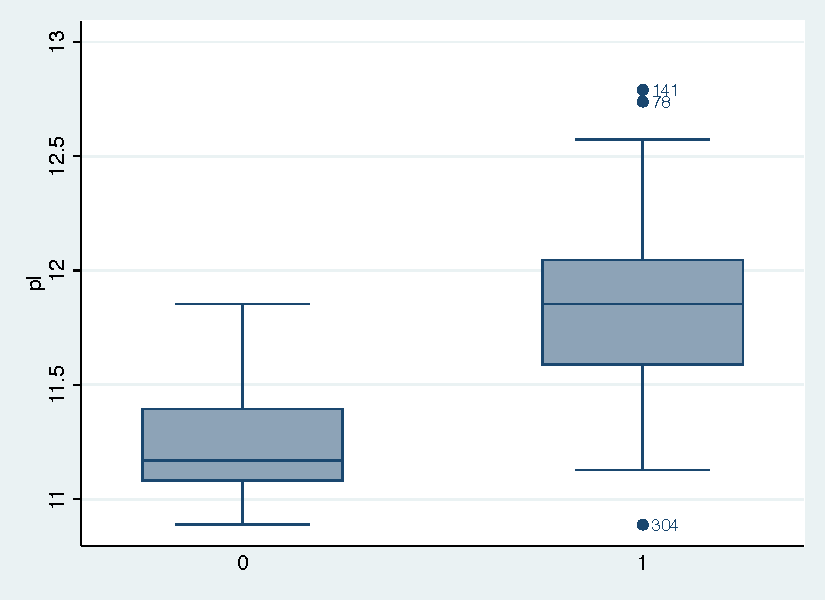
\includegraphics[width=.9\linewidth]{figures/cac-box.pdf}
  \caption{Central Air}
  \label{fig:cac-box}
\end{figure}

%--

\subsection*{Condition}
I had high hopes for this but it has some serious trouble (Figure~\ref{fig:condition-scatter}.
Note the scores for $condition=5$:
We see nice, similar-ish variances for the other conditions, gradually creeping up in price.
Perhaps someone thought the scale was 1-5, or there was some other data error. 
I will introduce a hack, recoding 1=3, 2=4, 3=6, 4=7 and 5=5,8,9 and call it recond,
then break that up into bar1-5. 
\begin{figure}[H]
\centering
  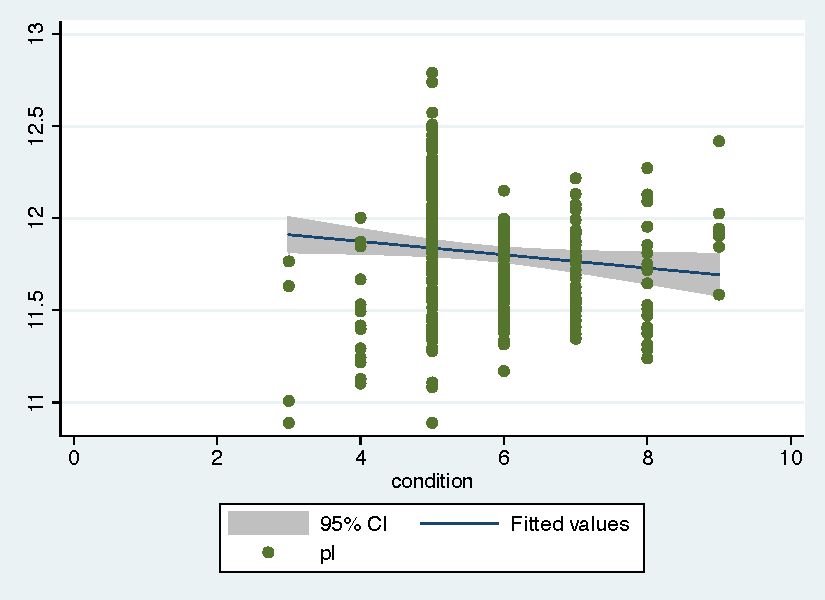
\includegraphics[width=.9\linewidth]{figures/condition-scatter.pdf}
  \caption{Condition}
  \label{fig:condition-scatter}
\end{figure}

%--

\subsection*{Basement Square Feet}
I had high hopes for this one.
A continuous variable with not many outliers (Figure~\ref{fig:basement-box}),
exploratory regressions show it loves to generate heteroscedasticity.
It also failed Stata's ovtest, so 
I tried a number of transforms, partitioning the basement sizes using ttest ... , by(), etc.,
all to no avail.
We'll see how it affects heteroscedasticity in the multiple regression model:
if we see heteroscedasticity in that model, we'll pull basement and see what improvements we get.
\begin{figure}[H]
\centering
  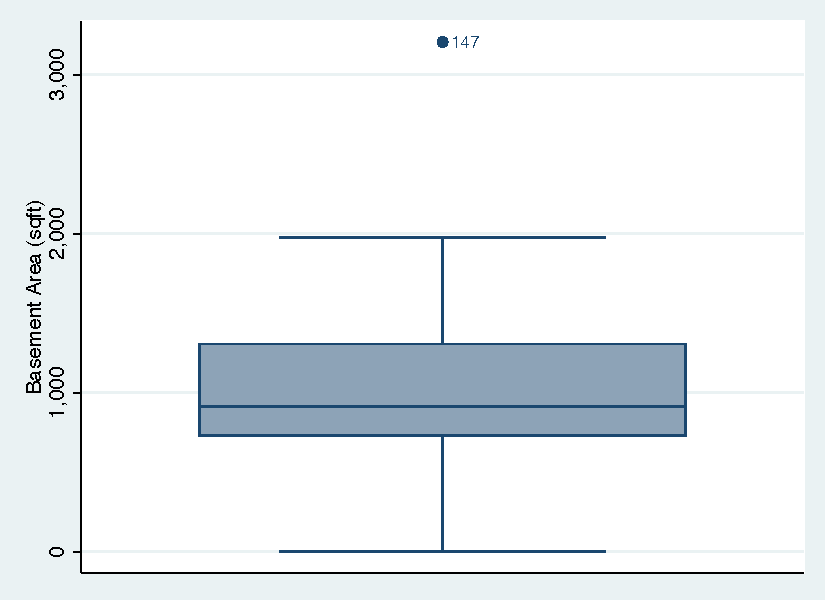
\includegraphics[width=.9\linewidth]{figures/basement-box.pdf}
  \caption{Basement Square Feet}
  \label{fig:basement-box}
\end{figure}

%--

\subsection*{Lot Size}
Another continuous variable with high hopes, the box plot (Figure~\ref{fig:lotSize-box}) shows some problems.
Attempts at tranformations (ln, etc.) did not help.
Attempts at dealing with outliers resulted in exacerbated skewness,
and while not terrific at nearly $0.77$, it is less than $0.8$.
I was able to remove four worst from these diagrams by selecting $lotSize > 19000$.
One off the cuff test was a ttest of lot sizes between our modeling building set of data and our kaggle data:
Stata says the $\mu$ of lot size in the Kaggle data is smaller.
This supports the decision to model without the larger lots,
hopefully trading overall accuracy of the model
for a model that will guess better at the unknown observations I have in front of me.
\begin{figure}[H]
  \centering
  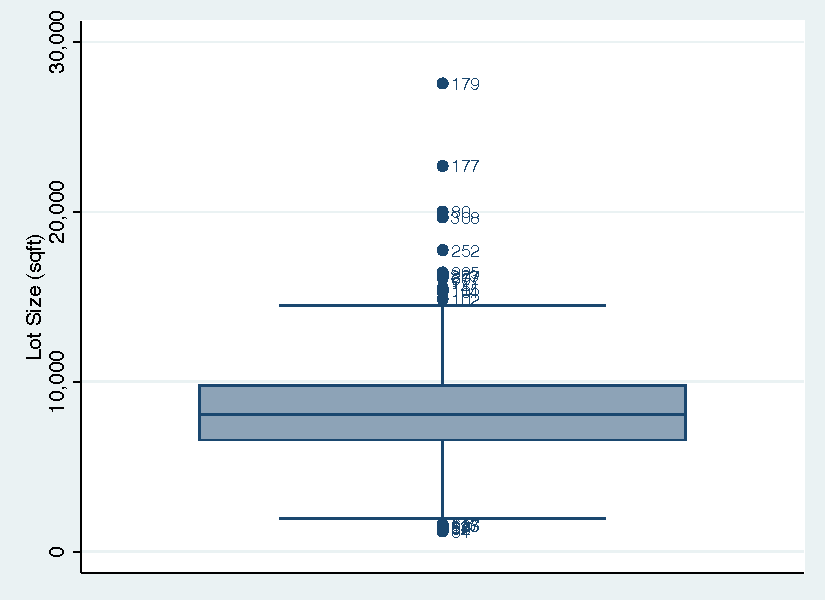
\includegraphics[width=.9\linewidth]{figures/lotSize-box.pdf}
  \caption{lotSize Box}
  \label{fig:lotSize-box}
\end{figure}

%--

\subsection*{Living Area}
A continuous variable that looks good (Figure~\ref{fig:sqft-box}),
exploratory regressions show it failed Stata's ovtest.
You can see that it doesn't fit well to the normal distribution shown in Figure~\ref{fig:sqft-qnorm}.
I eventually transformed this using square root,
which seems to generate a better model even though it still doesn't quite pass the ovtest.
sktest reports both are not normally distributed;
we'll serve up the less doctored one in the final dish and experiment with the transformed if it doesn't work well.
\begin{figure}[H]
\centering
  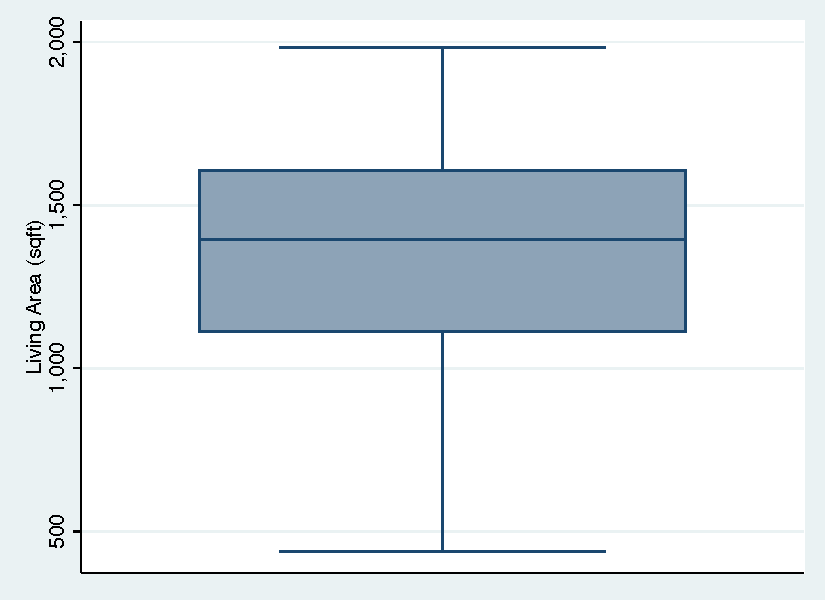
\includegraphics[width=.9\linewidth]{figures/sqft-box}
  \caption{Living Area}
  \label{fig:sqft-box}
\end{figure}
\begin{figure}[H]
\centering
  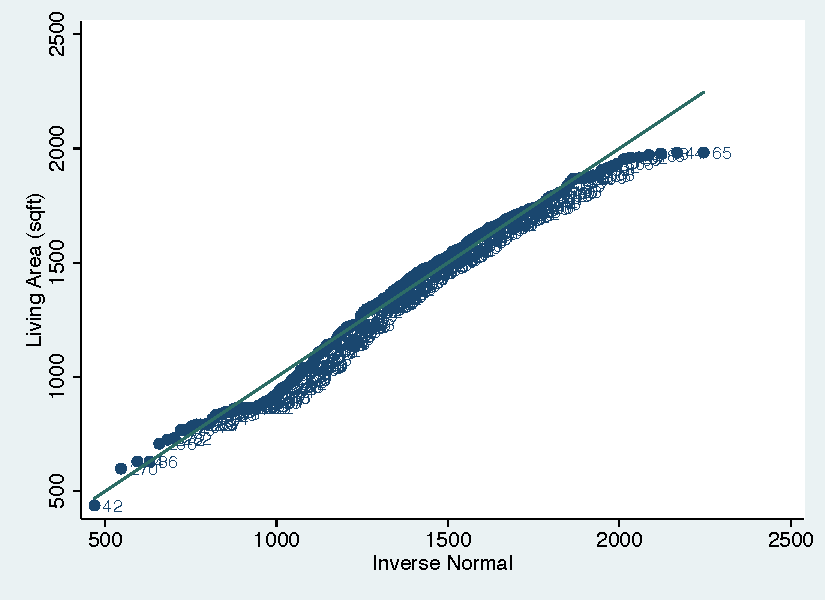
\includegraphics[width=.9\linewidth]{figures/sqft-qnorm.pdf}
  \caption{Living Area, normal distribution?}
  \label{fig:sqft-qnorm}
\end{figure}

%--

\subsection*{Deck}
Everyone loves a deck, no?
Alas, another continuous variable but no real correlation with price (Stata reports a correlation $<0.27$).
The variation on this variable is particularly screwy,
in particular note the variance on ``no deck'' spans all prices (Figure~\ref{fig:deck-scatter}).
\begin{figure}[H]
  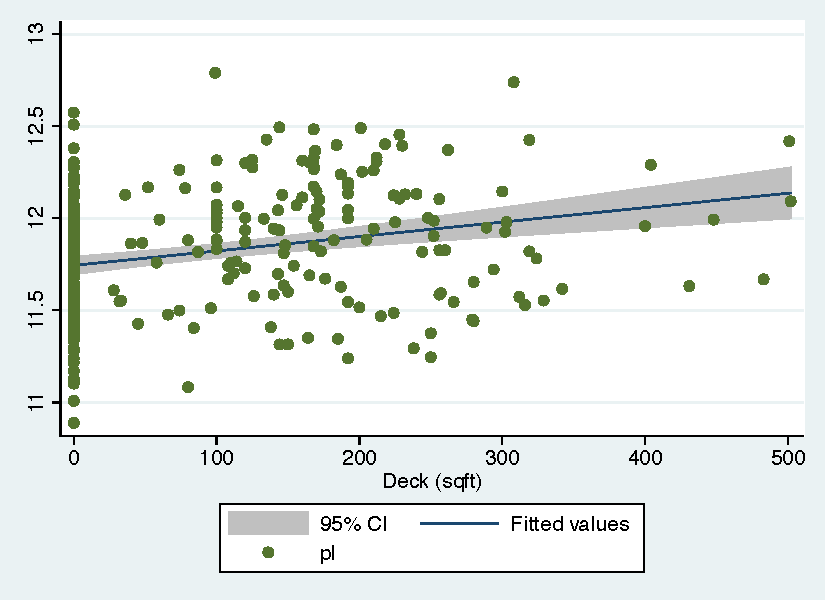
\includegraphics[width=.9\linewidth]{figures/deck-scatter}
  \caption{deck scatter}
  \label{fig:deck-scatter}
\end{figure}

%--

\subsection*{Miscellaneous}
A scatter plot of $distFire$, the distance to the fire department,
shows an amorphous blob.
Stata reports a correlation between $distFire, pl$ of $-0.0559$;
we can safely ignore this variable.
Likewise, Stata's ttest fails to reject the null hypothesis
that there's no difference for prices by $smoker$; the correlation with price is $0.0572$. Pass.

%--


\subsection*{Recap}
This feels like the junk food challenge on Top Chef,
since much of the data is skewed or has strange associations with our dependent variable.
We'll cobble together some recipes and see what we can serve up.

%----------------------------->8   Section   >8---------------------------------

\section*{Kitchen Sink}
Now throw it all into one large regression.
After the first iteration,
work to exclude residuals with an absolute value $>2$ and influential observations via Cook's Distance,
then rerun.
We get a pretty good run, all things considered, with Listing~\ref{fig:sink-log}.
The p-value (Prob $>$ F) is $<0.0001$, so we need at least some of our variables in the model.
Each variable is confirmed by its respective p-value $<0.05$.
$r^2 = 0.8814, r^2 adjusted = 0.8765$: This model accounts for 88.14\% of the variability in $pl$,
and $r^2 adjusted$ being close to $r^2$ tells us that this isn't just because we tossed a lot of
ingredients into the blender.
$s_e = 0.10754$, still within spitting distance of what I was
able to achieve with some questionable experiments.

Looking to the residuals, we observe that 3.2\% of our standardized residuals are greater than two standard deviations
from our prediction, we'd expect up to 5\%.
$H_0: \text{Residuals are normally distributed}; H_a: \text{Residuals are not normally distributed}$,
Stata's Skewness/Kurtosis test reports a p-value of 0.1282.
We fail to reject the null hypothesis, our residuals look to be normally distributed,
confirming one assumption of regression. We also test $H_0: \text{The model fits a straight line}; H_a: \text{The model fits some other line}$.
Stata's Ramsey Reset test reports a p-value of 0.2675, we fail to reject the null hypothesis
and confirm another assumption of regression.

Finally we test for heteroscedasticity.
$H_0: \text{Variance is constant across predicted values}; H_a: \text{variance is not constant}$,
Stata's Breusch-Pagan / Cook-Weisberg test reports a p-value of 0.3771,
again we fail to reject and this model looks good.

There are some troubles.
First, there are a lot of variables. And a lot of this data is past its sell-by date.
We also had to cull a lot of observations--nearly 70 of 320.
The MAE score for modeled data was roughly 12,000, but non-modeled data rolled in over 20,000.
Finally, there are a lot of variables in this model to explain and some of them ($br$)
have nonintuitive explanations to make.
I pass.

\begin{figure}[H]
\centering
  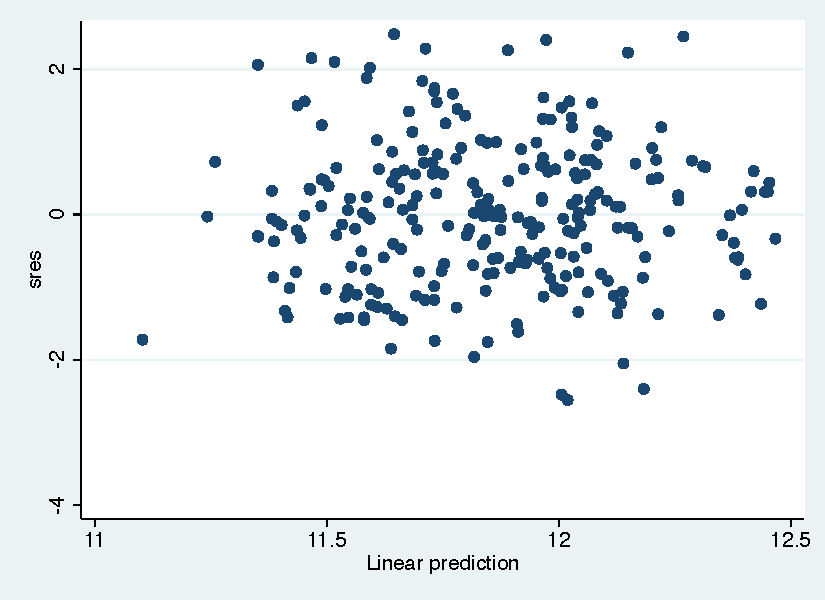
\includegraphics[width=.9\linewidth]{figures/reg-man-rvf}
  \caption{Residuals vs. Fit for Candidate}
  \label{fig:reg-man-rvf}
\end{figure}
\begin{figure}[H]
\centering
  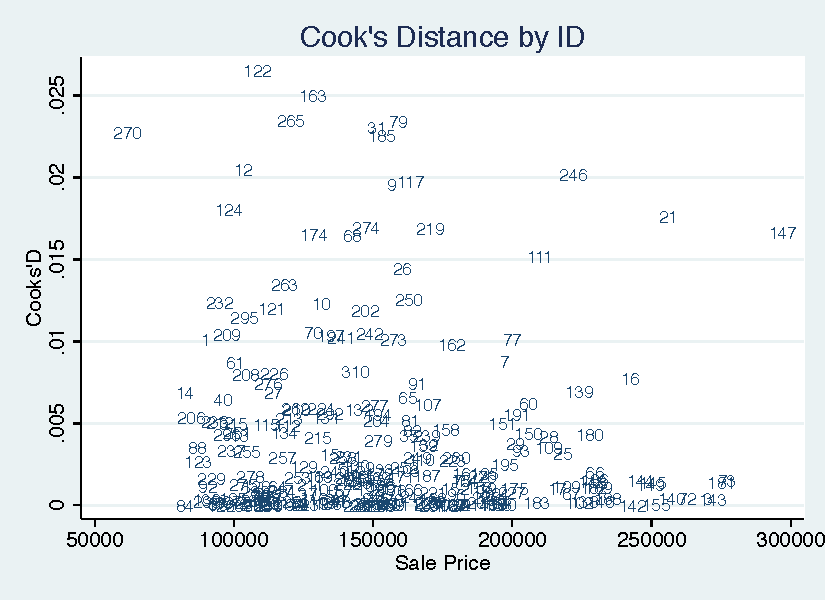
\includegraphics[width=.9\linewidth]{figures/reg-man-cooked}
  \caption{Cooks Distance for Candidate}
  \label{fig:reg-man-cooked}
\end{figure}

%----------------------------->8   Section   >8---------------------------------

\section*{Good Knife Work?}
So I decided to make my own regression choices and attempt to find a more parsimonious model.
One thing I was hoping to not lose so many observations to outliers in predictor variables.
There was some initial success as I had 18 more observations to start,
but 10 came back out after looking at Cook's Distance and large residuals ($>2.5$).
Still, I removed less than 20\% but still a lot.

%--

\subsection*{Technical Analyis}
Technically, the model is sound, noted in Listing~\ref{fig:model-reg}.
The p-value (Prob $>$ F) is $<0.0001$, so we need at least some of our variables in the model.
Each variable is confirmed by its respective p-value $<0.05$.
$r^2 = 0.8367, r^2 adjusted = 0.8327$: This model accounts for 83.67\% of the variability in $pl$,
and $r^2 adjusted$ being close to $r^2$ reassures us again.
$s_e = 0.12475$, still within spitting distance of our sink model and what I was
able to achieve with some questionable experiments.

5.4\% of our standardized residuals (Figure~\ref{fig:reg-man-rvf}) were greater than two,
casting some niggling doubt on the predictive power of our model.

$H_0: \text{Residuals are normally distributed}; H_a: \text{Residuals are not normally distributed}$,
Stata's Skewness/Kurtosis test reports a p-value of 0.5008.
We fail to reject the null hypothesis, our residuals look to be normally distributed,
confirming one assumption of regression. We also test $H_0: \text{The model fits a straight line}; H_a: \text{The model fits some other line}$.
Stata's Ramsey Reset test reports a p-value of 0.5875, we fail to reject the null hypothesis
and confirm another assumption of regression.

Finally we test for heteroscedasticity.
$H_0: \text{Variance is constant across predicted values}; H_a: \text{variance is not constant}$,
Stata's Breusch-Pagan / Cook-Weisberg test reports a p-value of 0.2974,
again we fail to reject and this model looks good.

%--

\subsection*{Interpretation}
Our model predicts the natural log ($x$) of $salesprice$:

\begin{math}
x = 11.01223 - 0.1221579 \times aget +
0.0205386 \times sqftt +
0.1141497 \times bar4 +
0.0000216 \times lotsize +
0.0466525 \times fpp +
0.1355746 \times garage
\end{math}

Finally, $salesprice = e^x$.

It can be interpreted as follows:
The sale price of a brand new house on an infinitesimally small lot with no living space,
panned for its condition, no fireplace, no garage would be $e^{11.01223}=\$60,610.90$, on average.
For every 1\% increase in age, while all other variables remaining the same, the price of the house decreases 12.2\%, on average.
As square feet increase by squares (${1,4,9,16,25,\ldots}$), while all other variables remaining the same, the price of the house increases 2.05\%, on average.
For each unit increase in condition, while all other variables remaining the same, the price of the house increases 11.41\%, on average.
For each additional square foot in the size of the lot, while all other variables remaining the same, the price of the house increases 0.0022\%, on average.
Fireplaces will add 4.66\% to the price of the house, on average, all other variables remaining the same.
Each additional garage space adds 13.56\% to the price of the house, on average, all other variables remaining the same.

Creating the the CI for this estimate is a little more difficult.
It's still $\pm 1.96 \times 0.12475$ but this is to the natural log,
the actual CI will be asymmetric because you adding/subtracting to the exponent of e.
The lower bound will be closer to the estimate than the upper bound.

%--

\subsection*{Notes and Caveats}
I did predict for a 100 year 200 sqft house on a 500 sqft lot with nothing and got a prediction \$$42,844$.

I would like to research and understand better the idea of a percentage increase for things like ``if fireplaces'' and garage spots. This seems to run a counter to what I've seen.

This model predicts meh for observations from the model, with a MAE of $14,224$,
and less than meh for observations not from the model, a MAE of $28036$ from the model data that I dropped, 
and $17,269$ for the Kaggle data.

The model seems rotated counter-clockwise.
I found the median sale price and counted the large residuals ($>2, <2$)
by price greater and price less than.
I see that for prices less than the median,
gross underestimates outnumber the overestimates 15-4.
For prices greater, the overestimates win 13-5\footnote{Using all modeling building data,
whether I actually included it in my regression model or not.}

Armed with this knowledge and some healthy skepticism with regard to overfitting,
I would prefer this model to the stepwise model shown earlier.

%---------------------------->8   Appendixes   >8--------------------------------

\onecolumn

%--

\lstinputlisting[label=fig:sink-log,caption={Stepwise Multiple Regression, Kitchen Sink}]{figures/sink-log.txt}

%--

\pagebreak\lstinputlisting[label=fig:model-reg,caption={Manual Multiple Regression}]{figures/reg-man-reg.txt}

%--

\pagebreak
\begin{table}[scale=0.4]
\caption{Data Description}
\label{tab:data}
\centering
\begin{tabular}{lll}
\hline
Variable   & Original           & Description \\
\hline
ID         &                    & data driven observation ID \\
salesprice &                    & Selling price in dollars \\
pl         & new transform      & natural log of salesprice \\
\hline
sqft       & live\_area\_sqft   & Square footage of living space \\
sqftt      & new transform      & $\sqrt{sqft}$ \\
basement   & bsmt\_sf           & Square footage of basement \\
lotSize    & lot\_sq\_ft        & Size of lot in square feet \\
lotSizet   & new transform      & ln of lotSize \\
deck       & deck\_sf           & Size of deck in square feet \\
dp         & new dummy          & $deck > 50$ square feet? \\
\hline
age        &                    & Age of the house in years \\
aget       & new transform      & natural log of age \\
distFire   &                    & Distance from the closest fire station \\
\hline
baths      &                    & Count of bathrooms \\
bedrooms   &                    & Count of bedrooms \\
fp         & fireplaces         & Count of fireplaces \\
fpp        &                    & Has one or more fireplaces \\
garage     & garage\_cars       & Count of spaces in garage \\
\hline
condition  &                    & Rated conditon 1-10 \\
recond     & recode             & Recoded condition, 1-5 \\
bar$n$     & recode             & Indicators for recode \\
cac        &                    & Boolean, central air \\
smoker     &                    & Boolean, previous owner smoked \\
monthSold  & month\_sold        & Month of year sold 1-12 \\
\hline
\end{tabular}
\end{table}

%--

\end{document}



